\documentclass[11pt,a4paper]{article}
\usepackage[margin=2.2cm]{geometry}
\usepackage{amsmath,amssymb}
\usepackage{booktabs}
\usepackage{array}
\usepackage{float}
\usepackage{graphicx}
\usepackage[font=small,labelfont=bf]{caption}
\usepackage{microtype}
\usepackage{xcolor}
\usepackage[colorlinks=true,linkcolor=blue!60!black,citecolor=blue!60!black,urlcolor=blue!60!black]{hyperref}

\newcommand{\zH}{\zeta_H}
\newcommand{\mom}[1]{\langle #1\rangle}
\newcommand{\qqq}{q(qq)}

\title{Nucleon distribution functions from the quark\,+\,diquark Faddeev amplitude:\\ results}
\author{Zhen-Ni Xu}
\date{23 November 2026 \quad (notes for discussion)}

\begin{document}
\maketitle

\section*{Summary}
\begin{itemize}
\item Valence DFs of the proton are computed directly from the \emph{solved} quark\,+\,diquark Faddeev amplitude of
  Ref.~\cite{Cheng:2026gff} (no ansatz for the hadron-scale wave function), through Mellin moments $\mom{x^m}$ of the
  light-front-weighted forward currents. Reliable moments reach $m \approx 9$--$10$.
\item Exact checks hold: $u$ and $d$ numbers $2,1$ to $4\times10^{-5}$; momentum sum $0.99996$; $\mom{x}_q = A^q(0)$
  of our gravitational form factors to $0.1\%$; an independent Fortran implementation agrees to $\le 7\times10^{-9}$.
\item After all-orders (AO) evolution, the valence moments at $\zeta_3 = 3.097$~GeV agree with the realistic CSM
  results of Ref.~\cite{Lu:2022cjx} within their errors; the symmetry-preserving contact interaction (SCI) is
  10--35\% harder in $\mom{x^2}$, $\mom{x^3}$.
\item At 2~GeV, $\mom{x}$ agrees with global fits to 2\%; the valence $\mom{x^2}_{u^- - d^-} = 0.050$ is about 11\% below
  global fits (and well below recent lattice results).
\item Helicity DFs with the symmetry-preserving axial current: $g_A = 1.157$ (9\% below experiment),
  $\Delta u/g_A = 0.777$, $\Delta d/g_A = -0.223$; $\mom{x}_{\Delta u - \Delta d}(2\,\text{GeV}) = 0.198$, in line with
  global fits.
\item Spin budget at $\zeta_C = \sqrt{3}$~GeV: measured quark helicity $a_0^E = 0.32$--$0.33$ (COMPASS 0.32(7));
  $\Delta G = 1.27$--$1.32$, in tension with lattice.
\end{itemize}

\section{Setup in brief}
Framework and parameters as in Ref.~\cite{Cheng:2026gff}: algebraic dressed-quark propagator, scalar and axial-vector
diquarks ($m_{0^+} = 0.79$, $m_{1^+} = 0.89$~GeV), Faddeev equation solved numerically, $M_N = 1.1787$~GeV.
Moments $\mom{x^m}_q = \mathrm{Tr}[n\cdot J^{(m)}_q]/\mathrm{Tr}[n\cdot J^B]$ with $n^2 = 0$, all forward-current
diagrams included (quark, diquark, exchanged quark, seagulls), canonical normalisation from $d\lambda/dM$.
Quark-in-diquark DFs from the squared diquark DAs as in Refs.~\cite{EPJC84:739,Yu:2025sci}. Higher moments use the
regulator $(1+\lambda p^2)^{-m}$ of Ref.~\cite{Bednar:2018mtf}, extrapolated to $\lambda \to 0$. Evolution: AO scheme
with the process-independent charge; $\zH = 0.3266$~GeV (nominal 0.331) reproduces $\mom{x}_\text{val} = 0.477$
(2~GeV) and 0.441 (3.097~GeV) of Refs.~\cite{EPJC84:739,Yu:2025sci}.

\section{Hadron-scale valence moments}
\begin{table}[H]
\centering\footnotesize
\setlength{\tabcolsep}{3.5pt}
\begin{tabular}{l*{11}{c}}
\toprule
$m$ & 0 & 1 & 2 & 3 & 4 & 5 & 6 & 7 & 8 & 9 & 10\\
\midrule
$\mom{x^m}_u$ & 1.99992 & 0.68726 & 0.27398 & 0.12146 & 0.05823 & 0.02971 & 0.01595 & 0.00896 & 0.00528 & 0.00320 & 0.00215\\
$\mom{x^m}_d$ & 0.99996 & 0.31271 & 0.11565 & 0.04838 & 0.02191 & 0.01058 & 0.00538 & 0.00287 & 0.00154 & 0.00079 & --\\
\bottomrule
\end{tabular}
\caption{Valence moments at $\zH$. Uncertainty $\le 1\%$ up to $m = 8$ ($\lambda$-extrapolation spread),
3--5\% at $m = 9$--$10$. Beyond $m \approx 10$ the terms containing the axial-diquark propagator and the two-loop
diagrams become unstable.}
\end{table}

\begin{itemize}
\item Per $u$ quark, $\mom{x^2}/\mom{x^0} = 0.137$ (SCI: about 0.151): our hadron-scale DFs are narrower.
\item Large $x$: $(1-x)^\beta$ with $\beta = 3$ fits all moments $m \le 9$--$10$ ($\chi^2/\text{dof} \approx 1.1$--$1.2$);
  $\beta = 4, 5$ are disfavoured.
\item The per-quark ratio of $d$ to $u$ moments falls from 0.91 ($m = 1$) to 0.49 ($m = 9$) without levelling off, so
  $d/u(x\to1)$ is not yet determined. (Bednar, Clo\"et and Tandy~\cite{Bednar:2018mtf} quote $0.087\pm0.010$ from 20
  moments in a rainbow-ladder q(qq) calculation.)
\end{itemize}

\section{Quark-in-diquark distributions}
\begin{table}[H]
\centering\small
\begin{tabular}{lcccc}
\toprule
 & $\mom{\xi^2}$, $\mom{\xi^4}$, $\mom{\xi^6}$ of $\phi_D$ & DA fit $\alpha$, $a_2$, $a_4$ & $\mom{z^2}$, $\mom{z^3}$, $\mom{z^4}$ of $\phi_D^2$\\
\midrule
$0^+$ & 0.1901, 0.0755, 0.0393 & 1.61, $-0.005$, $-0.025$ & 0.2850, 0.1775, 0.1177\\
$1^+$ & 0.1090, 0.0307, 0.0124 & 3.36, $-0.010$, $+0.005$ & 0.2653, 0.1480, 0.0861\\
asymptotic $6x(1-x)$ & 0.2, 0.0857, 0.0476 & 1.5, 0, 0 & 0.2857, 0.1786, 0.1190\\
\bottomrule
\end{tabular}
\caption{Diquark leading-twist DAs ($\xi = 2x-1$) computed from our diquark amplitudes,
$\phi(x) = N[x(1-x)]^{\alpha-1/2}[1 + a_2C_2^\alpha + a_4C_4^\alpha]$, and the resulting quark-in-diquark DF moments.
The $1^+$ DA is narrow; the two-parameter form cannot reach it. Two- vs three-parameter fits change the proton
moments by $< 0.2\%$.}
\end{table}

\section{Evolved moments}
\begin{table}[H]
\centering\small
\begin{tabular}{lccc}
\toprule
 & this work & SCI~\cite{EPJC84:739} & realistic CSM~\cite{Lu:2022cjx}\\
\midrule
$\mom{x}_u$, $\mom{x^2}_u$, $\mom{x^3}_u$ & 30.28, 7.61, 2.43 & 30.2, 8.4, 3.1 & 30.4(1.3), 7.7(5), 2.5(2)\\
$\mom{x}_d$, $\mom{x^2}_d$, $\mom{x^3}_d$ & 13.78, 3.21, 0.97 & 13.9, 3.7, 1.3 & 13.8(6), 3.2(2), 0.9(1)\\
$u-d$ & 16.50, 4.40, 1.46 & 16.4, 4.7, 1.8 & 16.6(7), 4.5(3), 1.6(1)\\
\bottomrule
\end{tabular}
\caption{Valence moments (\%) at $\zeta_3 = 3.097$~GeV. Same AO evolution in all three columns, so the comparison is of
the hadron-scale input: an ansatz in Ref.~\cite{Lu:2022cjx}, the solved Faddeev amplitude here.}
\end{table}

\begin{table}[H]
\centering\small
\begin{tabular}{llccccccc}
\toprule
 & & $u_V$ & $d_V$ & $g$ & $2\bar u$ & $2\bar d$ & $s+\bar s$ & $c+\bar c$\\
\midrule
$\mom{x}$ & this work & 32.8 & 14.9 & 41.5 & 2.58 & 3.74 & 3.16 & 1.33\\
 & SCI~\cite{Yu:2025sci} & 32.7 & 15.0 & 41.4 & 3.29 & 4.19 & 2.48 & 0.85\\
$\mom{x^2}$ & this work & 8.62 & 3.64 & 2.41 & 0.116 & 0.212 & 0.164 & 0.059\\
 & SCI & 9.47 & 4.15 & 2.67 & 0.175 & 0.258 & 0.136 & 0.040\\
$\mom{x^3}$ & this work & 2.84 & 1.13 & 0.389 & 0.015 & 0.030 & 0.023 & 0.008\\
 & SCI & 3.58 & 1.54 & 0.500 & 0.027 & 0.043 & 0.021 & 0.006\\
\bottomrule
\end{tabular}
\caption{All partons at $\zeta_2 = 2$~GeV (\%). Glue and total sea follow from the valence input and the evolution and
are reliable; the sea flavour split depends on the threshold and Pauli-term implementation (Sect.~\ref{sec:open}).}
\end{table}

\begin{table}[H]
\centering\small
\begin{tabular}{lccc}
\toprule
 & this work & global fits & lattice\\
\midrule
$\mom{x}_{u^+-d^+}$ & 0.167 & 0.155(5)~\cite{Butterworth:2015oua}; 0.161(18)~\cite{Lin:2017snn} & 0.173(14)(07)~\cite{Mondal:2020cmt}\\
$\mom{x}_{u^+}$ & 0.354 & 0.347(5)~\cite{Lin:2017snn} & --\\
$\mom{x}_{d^+}$ & 0.187 & 0.193(6)~\cite{Lin:2017snn} & --\\
$\mom{x}_{g}$ & 0.415 & 0.414(9)~\cite{Lin:2017snn} & 0.427(92)~\cite{Alexandrou:2020sml}\\
$\mom{x^2}_{u^--d^-}$ & 0.050 & 0.0562(11)~\cite{Ball:2021leu}; 0.0556(15)~\cite{Bailey:2020ooq} & 0.0814(50)~\cite{Alexandrou:2026gff}; 0.083(14)~\cite{Taggi:2026}\\
$\mom{x^2}_{u^-}$ & 0.086 & -- & 0.119(6)~\cite{Alexandrou:2026gff} (connected)\\
$\mom{x^2}_{d^-}$ & 0.036 & -- & 0.036(7)~\cite{Alexandrou:2026gff} (connected)\\
$\mom{x^3}_{u^+-d^+}$ & 0.017 & -- & 0.043(8)~\cite{Alexandrou:2026gff}\\
\bottomrule
\end{tabular}
\caption{Comparison at 2~GeV in the lattice conventions: $\mom{x}$, $\mom{x^3}$ for $q^+ = q + \bar q$,
$\mom{x^2}$ for $q^- = q - \bar q$. Ours: AO scheme, leading-order evolution; fits and lattice:
$\overline{\text{MS}}$ at 2~GeV, so scheme differences of a few per cent are possible for the higher moments.
NNPDF4.0 and MSHT20 values as quoted in Ref.~\cite{Taggi:2026}.}
\end{table}

\section{Dependence on $x$}
\begin{figure}[H]
\centering
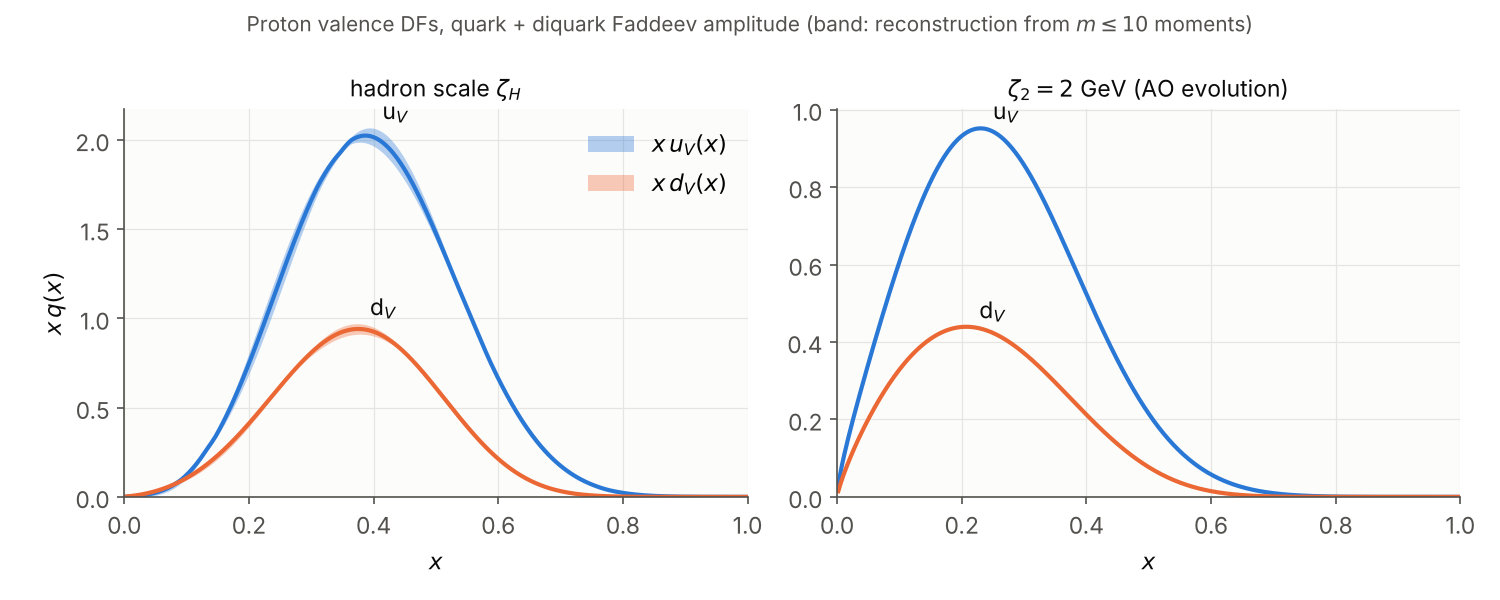
\includegraphics[width=\textwidth]{pdf_valence.png}
\caption{Valence DFs $x u_V(x)$, $x d_V(x)$ at $\zH$ (left) and at 2~GeV (right). Band: envelope of positive
fits ($N x^a (1-x)^b$, optionally $\times e^{cx + dx^2}$) to the moments $m \le 10$; it is reliable for
$0.15 \lesssim x \lesssim 0.7$ and understates the end-point uncertainty. The 2~GeV curves are refits of evolved moments,
not $x$-space evolution, so their small-$x$ behaviour is not meaningful.}
\end{figure}
Peaks at $\zH$: $x u_V \approx 2.0$ at $x \approx 0.39$; $x d_V \approx 0.94$ at $x \approx 0.38$.

\section{Helicity distributions}
\begin{table}[H]
\centering\footnotesize\setlength{\tabcolsep}{4pt}
\begin{tabular}{lccc}
\toprule
 & this work & Chen \emph{et al.}~\cite{Chen:2021guo} & Cheng \emph{et al.}~\cite{Cheng:2023kmt}\\
\midrule
$g_A$ & 1.157 & 1.25(3) & 1.25\\
$\Delta u/g_A$, $\Delta d/g_A$ & 0.777, $-0.223$ & $g_A^d/g_A^u = -0.16(2)$ & 0.762, $-0.238(6)$\\
$a_I/g_A = (\Delta u + \Delta d)/g_A$ & 0.553 & -- & 0.52(1)\\
\multicolumn{4}{l}{\emph{fraction of $g_A$ by diagram: 1 (scalar), 1 (axial), 2, 3, 4}}\\
 & 0.77, 0.071, 0.015, 0.075, 0.067 & 0.71, 0.064, 0.025, 0.13, 0.072 & --\\
\bottomrule
\end{tabular}
\caption{Axial charges at $\zH$ (experiment: $g_A = 1.2754$). Axial current of Ref.~\cite{Chen:2021guo} at $Q = 0$; the
diquark axial couplings are computed from the quark loop inside the diquark and used at each diquark's virtuality.
Ref.~\cite{Cheng:2023kmt} uses hadron-scale helicity DFs constrained by the axial charges; here they are computed.}
\end{table}

\begin{table}[H]
\centering\footnotesize
\setlength{\tabcolsep}{3.5pt}
\begin{tabular}{l*{10}{c}}
\toprule
$m$ & 0 & 1 & 2 & 3 & 4 & 5 & 6 & 7 & 8 & 9\\
\midrule
$\mom{x^m}_{\Delta u}$ & 0.8983 & 0.3360 & 0.1345 & 0.0579 & 0.0264 & 0.0128 & 0.0066 & 0.0036 & 0.0021 & 0.0012\\
$\mom{x^m}_{\Delta d}$ & $-0.2585$ & $-0.0797$ & $-0.0285$ & $-0.0110$ & $-0.0045$ & $-0.0020$ & $-0.0010$ & $-0.0005$ & $-0.0003$ & $-0.0002$\\
\bottomrule
\end{tabular}
\caption{Helicity moments at $\zH$.}
\end{table}

At 2~GeV (valence non-singlet evolution):
$\mom{x}_{\Delta u-\Delta d} = 0.198$ [NNPDFpol1.1 0.195(14)~\cite{Nocera:2014gqa}, DSSV08
0.203(9)~\cite{deFlorian:2009vb}, JAM17 0.241(26)~\cite{Ethier:2017zbq}, PNDME lattice
0.213(15)(22)~\cite{Mondal:2020cmt}];
$\mom{x^2}_{\Delta u-\Delta d} = 0.051$ [polarised fits 0.059--0.067, lattice 0.094(15)~\cite{Taggi:2026}]. The pattern is
the unpolarised one: $\mom{x}$ agrees, $\mom{x^2}$ is 15--20\% below fits.

\section{Gluon helicity and proton spin}
At $\zH$: $a_I = \Delta u + \Delta d = 0.640$, $\Delta G = \ell_g = 0$, quark orbital angular momentum
$\ell_q = \tfrac12 - \tfrac12 a_I = 0.180$. Light-front decomposition
$\tfrac12 = \tfrac12 a_I + \ell_q + \Delta G + \ell_g$, LO evolution with the AO charge as in
Refs.~\cite{EPJC84:739,Cheng:2023kmt}:
\begin{table}[H]
\centering\small
\begin{tabular}{lccccc}
\toprule
scale & $\tfrac12 a_I$ & $\ell_q$ & $\Delta G$ & $\ell_g$ & $a_I^E$\\
\midrule
$\zeta_C = \sqrt3$~GeV & 0.320 & $-0.023$ & 1.27--1.32 & $-1.07\ldots-1.11$ & 0.323--0.334\\
2~GeV & 0.320 & $-0.027$ & 1.39--1.43 & $-1.18\ldots-1.23$ & 0.319--0.329\\
$\sqrt{10}$~GeV & 0.320 & $-0.038$ & 1.75--1.81 & $-1.53\ldots-1.59$ & 0.307--0.317\\
\bottomrule
\end{tabular}
\caption{Spin budget; ranges from $\zH = 0.3266$ or 0.331~GeV. $a_I^E = a_I - n_f\,\alpha/(2\pi)\,\Delta G$ is the
measured (anomaly-corrected) quark helicity; COMPASS: $a_0(3\,\text{GeV}^2) = 0.32(7)$~\cite{Adolph:2016myg}.
Check of the implementation: with the input $a_0 = 0.65$ of Ref.~\cite{Cheng:2023kmt} we obtain
$\ell_q(\zeta_C) = -0.027$ (theirs $-0.027$), $\Delta G = 1.29$--$1.34$ (1.23), $a_0^E = 0.33$--$0.34$ (0.35(2)).}
\end{table}

\begin{itemize}
\item $\Delta G$ is large and positive, as in Ref.~\cite{Cheng:2023kmt}; the $\chi$QCD lattice glue spin
  $S_G = 0.251(47)(16)$ at $\mu^2 = 10$~GeV$^2$~\cite{Yang:2016plb} is much smaller. AO first moments include the small-$x$
  glue, and the definitions and schemes differ.
\item Quark orbital angular momentum by flavour at $\zH$ depends on the definition: light-front (Wandzura--Wilczek type)
  $\ell_u = -0.106$, $\ell_d = 0.286$; Ji, with our gravitational form factors, $L_u = 0.112$, $L_d = 0.047$. They differ by
  $B_q(0)/2$ with $B_u = 0.435$, $B_d = -0.477$; the WW split assumes $B_q = 0$ flavour by flavour.
\end{itemize}

\section{Open questions for discussion}\label{sec:open}
\begin{enumerate}
\item \textbf{Spin-flip deficit.} $A(0)$ and $D$ agree with Ref.~\cite{Cheng:2026gff} to 0.5\% and 1\%, but $J(0) = 0.479$
  (should be $\tfrac12$), $S(0)$, $\mu_p$, $\mu_n$ are 3--5\% low and $g_A$ is 9\% low. Resolution, grids, frame and
  diquark radii are ruled out; the transverse part of the quark vertex is suspected. A diagram-by-diagram comparison of
  $J(0)$ would settle it. The low $\mom{x^2}_u$ may have the same origin.
\item \textbf{AO thresholds.} Taken literally, the thresholds give glue 42.3\% and sea 9.5\% at 2~GeV; normalising them
  to $\sum_f \mathcal P^f_{qg} = 4$ gives 41.2\%/10.6\%, close to Ref.~\cite{Yu:2025sci} (41.4\%/10.8\%). The strange and
  charm fractions still differ (our $s+\bar s$ 3.2\% vs 2.5\%).
\item \textbf{Pauli term sign.} With $\sqrt3(1-2x)g_f$ and $g_d = +0.34$ as printed, momentum flows out of $d + \bar d$;
  we use the sign that gives $\bar d > \bar u$.
\item \textbf{Quark-in-diquark DFs.} The DA$^2$ approximation is used, with the longitudinal $1^+$ DA. Is a direct
  calculation of the diquark triangle worth it?
\item \textbf{Axial-diquark propagator at large momentum.} The $K_\mu K_\nu/m^2$ term does not fall off; terms with an
  axial-diquark propagator become unstable for $m \gtrsim 10$, and the axial-diquark light-front distribution
  $\mom{y^m}_{1^+}$ is negative for $m \ge 8$ (a model property, stable under all grid changes). Fixing $d/u(x\to1)$ needs
  $m \gtrsim 12$.
\item \textbf{Diquark axial couplings.} With the constant couplings $\kappa^{aa}_{ax} = 0.73$, $\kappa^{sa}_{ax} = 0.75$ of
  Ref.~\cite{Chen:2021guo}, our diagrams 2 and 3 are twice those of their table (flavour factors checked). How are
  these vertices normalised in your code?
\item \textbf{Publication.} Scope (unpolarised only, or with helicity and spin) and the relation to
  Ref.~\cite{Bednar:2018mtf}.
\end{enumerate}

\begin{thebibliography}{99}\small
\bibitem{Cheng:2026gff} P.~Cheng, Z.-N.~Xu, D.-Y.~Fu, C.~Chen, Z.-Q.~Yao, \emph{Quark\,+\,diquark description of nucleon
  gravitational form factors}, \href{https://arxiv.org/abs/2611.19819}{arXiv:2611.19819}.
\bibitem{EPJC84:739} Y.~Yu, P.~Cheng, H.-Y.~Xing, F.~Gao, C.~D.~Roberts, \emph{Contact interaction study of proton parton
  distributions}, Eur.\ Phys.\ J.\ C \textbf{84} (2024) 739, \href{https://arxiv.org/abs/2402.06095}{arXiv:2402.06095}.
\bibitem{Yu:2025sci} Y.~Yu \emph{et al.}, \emph{Distribution functions of $\Lambda$ and $\Sigma^0$ baryons},
  \href{https://arxiv.org/abs/2505.10663}{arXiv:2505.10663}.
\bibitem{Lu:2022cjx} Y.~Lu \emph{et al.}, \emph{Proton and pion distribution functions in counterpoint},
  Phys.\ Lett.\ B \textbf{830} (2022) 137130, \href{https://arxiv.org/abs/2203.00753}{arXiv:2203.00753}.
\bibitem{Bednar:2018mtf} K.~D.~Bednar, I.~C.~Clo\"et, P.~C.~Tandy, \emph{Nucleon quark distribution functions from the
  Dyson--Schwinger equations}, \href{https://arxiv.org/abs/1803.03656}{arXiv:1803.03656}.
\bibitem{Chen:2021guo} C.~Chen, C.~S.~Fischer, C.~D.~Roberts, J.~Segovia, \emph{Nucleon axial-vector and pseudoscalar form
  factors, and PCAC relations}, \href{https://arxiv.org/abs/2103.02054}{arXiv:2103.02054}.
\bibitem{Cheng:2023kmt} P.~Cheng \emph{et al.}, \emph{Polarised parton distribution functions and proton spin},
  Phys.\ Lett.\ B \textbf{844} (2023) 138074, \href{https://arxiv.org/abs/2304.12469}{arXiv:2304.12469}.
\bibitem{Butterworth:2015oua} J.~Butterworth \emph{et al.}, \emph{PDF4LHC recommendations for LHC Run II},
  \href{https://arxiv.org/abs/1510.03865}{arXiv:1510.03865}.
\bibitem{Lin:2017snn} H.-W.~Lin \emph{et al.}, \emph{Parton distributions and lattice QCD calculations: a community white
  paper}, Table~3.7, \href{https://arxiv.org/abs/1711.07916}{arXiv:1711.07916}.
\bibitem{Mondal:2020cmt} S.~Mondal \emph{et al.} (PNDME), \emph{Moments of nucleon isovector structure functions in
  2+1+1-flavor QCD}, \href{https://arxiv.org/abs/2005.13779}{arXiv:2005.13779}.
\bibitem{Alexandrou:2020sml} C.~Alexandrou \emph{et al.} (ETMC), \emph{Complete flavor decomposition of the spin and momentum
  fraction of the proton using lattice QCD simulations at physical pion mass},
  \href{https://arxiv.org/abs/2003.08486}{arXiv:2003.08486}.
\bibitem{Ball:2021leu} R.~D.~Ball \emph{et al.} (NNPDF), \emph{The path to proton structure at one-percent accuracy},
  \href{https://arxiv.org/abs/2109.02653}{arXiv:2109.02653}.
\bibitem{Bailey:2020ooq} S.~Bailey \emph{et al.}, \emph{Parton distributions from LHC, HERA, Tevatron and fixed target data:
  MSHT20 PDFs}, \href{https://arxiv.org/abs/2012.04684}{arXiv:2012.04684}.
\bibitem{Alexandrou:2026gff} C.~Alexandrou \emph{et al.} (ETMC), \emph{The nucleon unpolarized generalized form factors and
  Mellin moments up to fourth order}, \href{https://arxiv.org/abs/2607.03458}{arXiv:2607.03458}.
\bibitem{Taggi:2026} E.~Taggi, M.~Engelhardt, J.~R.~Green, \emph{Third moments of nucleon unpolarized, polarized, and
  transversity parton distribution functions from physical-point lattice QCD},
  \href{https://arxiv.org/abs/2605.02808}{arXiv:2605.02808}.
\bibitem{Nocera:2014gqa} E.~R.~Nocera \emph{et al.} (NNPDF), \emph{A first unbiased global determination of polarized PDFs
  and their uncertainties}, \href{https://arxiv.org/abs/1406.5539}{arXiv:1406.5539}.
\bibitem{deFlorian:2009vb} D.~de~Florian \emph{et al.}, \emph{Extraction of spin-dependent parton densities and their
  uncertainties}, \href{https://arxiv.org/abs/0904.3821}{arXiv:0904.3821}.
\bibitem{Ethier:2017zbq} J.~J.~Ethier \emph{et al.} (JAM), \emph{First simultaneous extraction of spin-dependent parton
  distributions and fragmentation functions from a global QCD analysis},
  \href{https://arxiv.org/abs/1705.05889}{arXiv:1705.05889}.
\bibitem{Adolph:2016myg} C.~Adolph \emph{et al.} (COMPASS), \emph{Final COMPASS results on the deuteron spin-dependent
  structure function $g_1^d$ and the Bjorken sum rule}, \href{https://arxiv.org/abs/1612.00620}{arXiv:1612.00620}.
\bibitem{Yang:2016plb} Y.-B.~Yang \emph{et al.} ($\chi$QCD), \emph{Glue spin and helicity in proton from lattice QCD},
  \href{https://arxiv.org/abs/1609.05937}{arXiv:1609.05937}.
\end{thebibliography}

\end{document}
